%==============================================================================
\section{Results}
\label{sec:results}

We organise the results into six subsections. Section~\ref{sec:results-main}
gives the main test-set leaderboard. Sections \ref{sec:results-boundary}
and \ref{sec:results-clinical} report boundary and clinical
(EF) metrics. Section~\ref{sec:results-robustness} examines robustness by
image quality. Section~\ref{sec:results-efficiency} reports the accuracy
$\times$ efficiency trade-off. Section~\ref{sec:results-significance}
reports statistical significance.

%------------------------------------------------------------------------------
\subsection{Main test-set Dice}
\label{sec:results-main}

Table~\ref{tab:main} summarises mean Dice, per-class Dice, and the
parameter count for each architecture on the official CAMUS test split.

%==============================================================================
% Paper 1 / T1 — Main Dice (auto-generated by fill_tables.py)
%==============================================================================
\begin{table*}[t]
\centering
\caption{Mean and per-class Dice on the CAMUS official test split for the
nine base architectures. The bracketed interval is the bootstrap 95\%
confidence interval on mean Dice over the 50-patient test set. Best per
column in \textbf{bold}, second-best \underline{underlined}. Per-class
scores are LV-endocardium, LV-epicardium, and left atrium.}
\label{tab:main}
\small
\setlength{\tabcolsep}{4pt}
\resizebox{\textwidth}{!}{%
\begin{tabular}{l c c c c c c c}
\toprule
Architecture       & Paradigm & {Mean Dice} & {95\% CI} & {LV-endo} & {LV-epi} & {LA} & {Params (M)} \\
\midrule
TransUNet          & Hybrid      & \textbf{0.9121} & [0.9078, 0.9162] & 0.9367 & 0.8789 & \textbf{0.9208} & 102.1 \\
nnU-Net            & CNN         & \underline{0.9099} & [0.9054, 0.9143] & \textbf{0.9371} & \textbf{0.8790} & 0.9136 &  15.6 \\
UNet-V1            & CNN         & 0.9085 & [0.9041, 0.9130] & 0.9369 & 0.8757 & 0.9129 &  31.0 \\
UNet-ResNet        & CNN         & 0.9081 & [0.9019, 0.9136] & 0.9341 & 0.8742 & 0.9160 &  29.1 \\
UNet-V2            & CNN         & 0.8963 & [0.8913, 0.9015] & 0.9239 & 0.8592 & 0.9059 &  33.0 \\
Swin-UNet          & Transformer & 0.8882 & [0.8829, 0.8936] & 0.9172 & 0.8520 & 0.8954 &  41.8 \\
DeepLabV3+         & CNN         & 0.8602 & [0.8511, 0.8681] & 0.9109 & 0.8187 & 0.8510 &  40.3 \\
FPN-UNet           & CNN         & 0.8596 & [0.8526, 0.8661] & 0.8962 & 0.7944 & 0.8881 &  32.2 \\
DenseContextU-Net  & CNN         & 0.8505 & [0.8414, 0.8604] & 0.8977 & 0.8046 & 0.8492 &   2.2 \\
\bottomrule
\end{tabular}}
\end{table*}


\paragraph{Headline ranking.}
\textbf{TransUNet} achieves the highest mean Dice ($0.9121$), narrowly
ahead of \textbf{nnU-Net} ($0.9099$, $\Delta = 0.0022$), \textbf{UNet-V1}
($0.9085$), and \textbf{UNet-ResNet} ($0.9081$). The four top architectures
are tightly clustered within $\Delta\text{Dice} \le 0.004$ ---
within the Bonferroni-corrected statistical-significance band
(Section~\ref{sec:results-significance}), so their ordering should not be
read as a ranking. Below this band,
\textbf{UNet-V2} ($0.8963$) and \textbf{Swin-UNet} ($0.8882$) form a
mid-tier, and \textbf{DeepLabV3+} ($0.8602$), \textbf{FPN-UNet}
($0.8596$), and \textbf{DenseContextU-Net} ($0.8505$) trail.

\paragraph{Per-class.}
LV-endo Dice ranges $0.8962$ (FPN-UNet) to $0.9371$ (nnU-Net);
LA Dice ranges $0.8492$ (DenseContextU-Net) to $0.9208$ (TransUNet);
LV-epi is consistently the hardest class for every architecture (mean
across models: $\Dice \approx 0.85$, versus $\approx 0.92$ for LV-endo).

Table~\ref{tab:iou} reports the same decomposition under intersection-over-union.
IoU orders the architectures almost identically to Dice, which is expected of two
monotonically related overlap measures; we report it because it is the more
common metric outside medical imaging and makes this benchmark comparable to
that literature.

%==============================================================================
% Paper 1 / T8 - Per-class IoU (auto-generated)
%   <- results/base_models/evaluation/evaluation_results.json : iou_*
%==============================================================================
\begin{table}[t]
\centering
\caption{Intersection-over-union on the CAMUS test split, mean and per
class. IoU orders the architectures almost identically to Dice, as expected
of two monotonically related overlap measures; it is reported because IoU is
the more common metric outside medical imaging and makes this benchmark
comparable to that literature. Best per column in \textbf{bold}.}
\label{tab:iou}
\small
\setlength{\tabcolsep}{6pt}
\begin{tabular}{l cccc}
\toprule
Architecture       & {Mean IoU} & {LV-endo} & {LV-epi} & {LA} \\
\midrule
TransUNet          & \textbf{0.8420} & 0.8828 & 0.7864 & \textbf{0.8570} \\
nnU-Net            & 0.8384 & \textbf{0.8833} & \textbf{0.7864} & 0.8456 \\
UNet-ResNet        & 0.8364 & 0.8790 & 0.7810 & 0.8493 \\
UNet-V1            & 0.8362 & 0.8828 & 0.7818 & 0.8441 \\
UNet-V2            & 0.8168 & 0.8610 & 0.7560 & 0.8335 \\
Swin-UNet          & 0.8037 & 0.8496 & 0.7447 & 0.8169 \\
DeepLabV3+         & 0.7657 & 0.8389 & 0.6980 & 0.7601 \\
FPN-UNet           & 0.7619 & 0.8142 & 0.6631 & 0.8085 \\
DenseContextU-Net  & 0.7513 & 0.8192 & 0.6783 & 0.7564 \\
\bottomrule
\end{tabular}
\end{table}


%------------------------------------------------------------------------------
\subsection{Boundary accuracy (HD95 and ASSD in mm)}
\label{sec:results-boundary}

Boundary metrics are reported in millimetres using the per-sample NIfTI
pixel spacing.

%==============================================================================
% Paper 1 / T2 — Boundary metrics in mm (auto-generated)
%==============================================================================
\begin{table}[t]
\centering
\caption{Boundary metrics on the CAMUS test split. HD95 is the
95\textsuperscript{th}-percentile Hausdorff distance, ASSD is the average
symmetric surface distance, both reported in millimetres using per-sample
NIfTI pixel spacing. Best per column in \textbf{bold}.}
\label{tab:boundary}
\small
\setlength{\tabcolsep}{6pt}
\begin{tabular}{l c c}
\toprule
Architecture       & {HD95 (mm)} & {ASSD (mm)} \\
\midrule
TransUNet          & \textbf{4.08} & \textbf{0.82} \\
UNet-ResNet        & 4.26 & 0.84 \\
nnU-Net            & 4.27 & 0.84 \\
UNet-V1            & 4.62 & 0.87 \\
Swin-UNet          & 5.08 & 1.00 \\
UNet-V2            & 5.29 & 1.03 \\
DeepLabV3+         & 5.71 & 1.19 \\
FPN-UNet           & 6.21 & 1.24 \\
DenseContextU-Net  & 8.29 & 1.55 \\
\bottomrule
\end{tabular}
\end{table}


\paragraph{HD95.}
TransUNet again leads with HD95 $= 4.08$~mm, followed by UNet-ResNet
($4.26$~mm) and nnU-Net ($4.27$~mm), UNet-V1 ($4.62$~mm), Swin-UNet
($5.08$~mm), and UNet-V2 ($5.29$~mm). All boundary distances are computed
at the native image resolution: CAMUS frames are approximately
$630 \times 519$ with a typical spacing of $0.308$~mm, so each prediction
is resampled back to its native grid before the distance transform is
taken. Measuring on the $256 \times 256$ network grid while applying the
native spacing would under-report every distance by the resampling factor
of $\sim$$2.2$, and we caution that this is an easy error to make silently.
The three best architectures sit within $0.2$~mm of one another
(TransUNet $4.08$, UNet-ResNet $4.26$, nnU-Net $4.27$), and the top four
within $0.54$~mm --- a spread well inside the training-variance floor
discussed in Section~\ref{sec:discussion}. All of them cluster around the
published CAMUS
nnU-Net baseline of $\approx 4.3$~mm \citep{leclerc2019}. Under a unified
modern protocol, then, boundary accuracy on CAMUS appears to have
saturated: our reproduction matches the 2019 baseline rather than
improving on it. That baseline was in any case reported under the original
CAMUS evaluation convention, which differs from our per-sample HD95, so
the cross-paper comparison is indicative rather than strictly
like-for-like.

\paragraph{ED versus ES.}
Table~\ref{tab:edes} reports ED- and ES-stratified mean Dice and HD95. The
two phases are closely matched for every architecture (mean Dice within
$\approx 0.007$ and HD95 within $\approx 1.4$~mm), with no consistent
advantage to either phase. This is a reassuring property for biplane EF, which
depends on both phases symmetrically.

%==============================================================================
% Paper 1 / T3 — ED/ES stratified (auto-generated)
%==============================================================================
\begin{table}[t]
\centering
\caption{End-diastole (ED) and end-systole (ES) stratified mean Dice and
HD95 (mm) on the CAMUS test split.}
\label{tab:edes}
\small
\setlength{\tabcolsep}{4pt}
\begin{tabular}{l c c c c}
\toprule
\multirow{2}{*}{Architecture} & \multicolumn{2}{c}{Dice} & \multicolumn{2}{c}{HD95 (mm)} \\
                              & {ED}   & {ES}   & {ED}   & {ES}   \\
\midrule
nnU-Net            & 0.9105 & 0.9093 & 4.19 & 4.35 \\
TransUNet          & 0.9105 & 0.9137 & 4.07 & 4.09 \\
UNet-V1            & 0.9072 & 0.9098 & 4.67 & 4.57 \\
UNet-ResNet        & 0.9062 & 0.9100 & 4.16 & 4.37 \\
UNet-V2            & 0.8989 & 0.8938 & 5.06 & 5.52 \\
Swin-UNet          & 0.8884 & 0.8880 & 5.02 & 5.14 \\
DeepLabV3+         & 0.8573 & 0.8631 & 5.67 & 5.76 \\
FPN-UNet           & 0.8559 & 0.8633 & 6.23 & 6.20 \\
DenseContextU-Net  & 0.8513 & 0.8497 & 7.61 & 8.98 \\
\bottomrule
\end{tabular}
\end{table}


%------------------------------------------------------------------------------
\subsection{Clinical metric: biplane Simpson's EF}
\label{sec:results-clinical}

Table~\ref{tab:ef} reports biplane Simpson's EF error per architecture.

%==============================================================================
% Paper 1 / T4 — EF metrics (auto-generated)
%==============================================================================
\begin{table}[t]
\centering
\caption{Biplane Simpson's ejection fraction (EF) metrics on the CAMUS
test set. Bias and the 95\% limits of agreement (LoA) are the
Bland--Altman statistics against reference EF over the 50 test patients.
Best per column in \textbf{bold}.}
\label{tab:ef}
\small
\setlength{\tabcolsep}{6pt}
\begin{tabular}{l c c c c}
\toprule
Architecture       & {MAE (\%)} & {$r$} & {Bias (\%)} & {95\% LoA (\%)} \\
\midrule
nnU-Net            & \textbf{5.52} & 0.828 & +0.84 & [-14.2, +15.9] \\
UNet-V1            & 6.78 & 0.793 & -0.74 & [-18.1, +16.6] \\
UNet-ResNet        & 6.78 & \textbf{0.832} & -2.42 & [-18.7, +13.8] \\
UNet-V2            & 7.60 & 0.728 & -1.20 & [-20.7, +18.3] \\
TransUNet          & 7.64 & 0.799 & -3.44 & [-21.4, +14.5] \\
DeepLabV3+         & 8.46 & 0.744 & -6.10 & [-24.0, +11.8] \\
FPN-UNet           & 10.12 & 0.677 & -8.12 & [-28.6, +12.4] \\
Swin-UNet          & 10.46 & 0.574 & -4.10 & [-31.0, +22.8] \\
DenseContextU-Net  & 16.04 & 0.444 & -11.52 & [-48.1, +25.0] \\
\bottomrule
\end{tabular}
\end{table}


\paragraph{Best EF agreement, and the floor beneath it.}
\textbf{UNet-V1} produces the most accurate EF estimates
(MAE $= 6.62\%$, Bland--Altman bias
$-0.42\%$), with TransUNet
(MAE $= 7.36\%$) and UNet-ResNet
(MAE $= 7.42\%$) close behind. Correlation separates them even
less: TransUNet attains the highest at $r = 0.826$, ahead of
UNet-V1's $0.825$, so the two lead on different EF statistics.

The informative row, however, is the last one. Passing the \emph{ground-truth}
masks through the identical pipeline gives MAE $= 5.44\%$ ($r = 0.863$), so no
architecture comes within $1.2$ points of the floor and none crosses it. That
residual is not a segmentation error: it is what biplane Simpson's method loses
when it reconstructs a three-dimensional ventricle from two views, plus the
disagreement between the clinically recorded EF and any mask-derived estimate.
Reported inter-observer LVEF error of $\sim$$7$--$10\%$ sits at the same scale,
which is the honest comparison to draw --- a like-for-like mask-derived
agreement, not a claim of clinical parity.

One qualification on the word ``floor''. The oracle carries a Bland--Altman
bias of $+3.12\%$: mask-derived EF systematically overestimates the recorded
clinical value, whatever the masks. Mean absolute error is therefore not
monotone in segmentation quality, because a model whose own bias runs the other
way has its errors partially cancel and can post a lower MAE without being more
faithful to the anatomy. The oracle bounds what \emph{perfect} masks achieve
under this estimator; it does not bound MAE in general. For the nine
architectures here the distinction is moot --- none approaches $5.44\%$, and
none exceeds the oracle's $r = 0.863$ either --- but any comparison that puts a
model at or under the oracle should be read on correlation and bias rather than
on MAE alone.

Read against that floor, EF separates architectures far less sharply than bulk
overlap does: the spread from best to worst is $4.0$ points on a quantity
whose irreducible component is $5.4$. The limits of agreement make the same
point per patient, spanning
$[-15.7, +14.8]\%$
even for the best model.

Two ordering effects survive and are worth stating. The best-Dice architecture
is not the best on the clinical axis --- TransUNet is second on EF --- and
nnU-Net, which leads no EF column, sits mid-table at $8.32\%$. The
Transformer-only Swin-UNet remains weak among the competitive models
($9.44\%$, $r = 0.640$) despite adequate bulk Dice,
consistent with contours that are locally plausible but systematically biased in
a way Simpson's integration compounds.

\paragraph{Arithmetic precision changes the EF table.}
Every EF value above is computed in full FP32. This is worth stating because it
is not the default: PyTorch enables TensorFloat-32 for convolution and matrix
multiplication on Ampere-class and later GPUs, and TF32 carries a 10-bit
mantissa against FP32's 23. We found that this silently changes the reported
result. Disabling TF32 moves FPN-UNet's EF MAE from $9.72$ to $10.60$ and
TransUNet's by $0.60$ --- differences larger than the gaps separating adjacent
architectures in this table.

We isolated the cause by ablating each control separately on one architecture.
Run-to-run variation with everything unpinned is only $0.02$ points; forcing
cuDNN determinism changes nothing at all; requiring deterministic algorithms
accounts for $0.28$; disabling TF32 accounts for the entire remaining shift.
The effect is not rounding. Twenty-six of the fifty test patients change, some
by as much as $14$ EF points and some end-diastolic volumes by around $20$~ml,
because a precision change flips pixels along an ambiguous basal boundary, the
largest-connected-component filter turns that into a discrete choice, and
Simpson's method needs all four of a patient's frames to score them at all.

FP32 is the more accurate computation, so the previously reported figures were
flattered by reduced precision rather than harmed by it.

With TF32 disabled and seeds fixed the pipeline becomes reproducible, and
markedly more portable than we expected. Independent runs in separate processes
return bit-identical values for all nine architectures. Repeating the
measurement on a different operating system, with a different PyTorch build
($2.10.0$ against $2.9.1$) and a different image-processing library version,
reproduces eight of the nine exactly; the ninth differs by $0.04$ percentage
points and the ranking is unchanged. Before pinning, the same cross-environment
comparison moved six of nine architectures and exchanged third and fourth place.
Arithmetic precision, not the software environment, was doing almost all of the
work.

We report this because a benchmark that does not state its arithmetic precision
is not reproducible even in principle, and because the effect here exceeds the
architectural differences the benchmark exists to measure. The practical
recommendation is one line of configuration: disable TF32 when reporting a
derived clinical quantity, and say that you did.

%------------------------------------------------------------------------------
\subsection{Robustness across image quality}
\label{sec:results-robustness}

CAMUS assigns each patient an expert image-quality grade (\emph{Good},
\emph{Medium}, \emph{Poor}). Table~\ref{tab:quality} reports mean Dice
stratified by that grade. Every architecture degrades monotonically from
Good to Poor, confirming that acquisition quality is a primary driver of
segmentation difficulty on CAMUS. The degradation is, however, markedly
gentler for the top-tier architectures: TransUNet and nnU-Net lose only
$\sim$$0.02$--$0.03$ Dice from Good to Poor and remain above $0.89$ on
Poor-quality frames, whereas the weakest models (DeepLabV3+,
DenseContextU-Net) drop by $0.04$ or more and fall below $0.83$.
Robustness to image quality therefore tracks overall accuracy rather than
trading off against it.

%==============================================================================
% Paper 1 / T5 -- quality-stratified Dice (auto-generated from
% quality_stratified.json produced by colab_session.py)
%==============================================================================
\begin{table}[t]
\centering
\caption{Mean Dice on the CAMUS test split stratified by the
expert-assigned image-quality grade (Good $n{=}94$, Medium $n{=}76$, Poor $n{=}30$ test frames). Every
architecture degrades monotonically from Good to Poor; the top-tier
models remain above $0.88$ even on Poor-quality images. Best per column
in \textbf{bold}.}
\label{tab:quality}
\small
\setlength{\tabcolsep}{6pt}
\begin{tabular}{l c c c}
\toprule
Architecture & {Good} & {Medium} & {Poor} \\
\midrule
TransUNet          & \textbf{0.9186} & 0.9097 & \textbf{0.8988} \\
nnU-Net            & 0.9168 & 0.9091 & 0.8903 \\
UNet-V1            & 0.9173 & 0.9070 & 0.8848 \\
UNet-ResNet        & 0.9156 & \textbf{0.9142} & 0.8734 \\
UNet-V2            & 0.9091 & 0.8921 & 0.8672 \\
Swin-UNet          & 0.8961 & 0.8866 & 0.8675 \\
FPN-UNet           & 0.8690 & 0.8628 & 0.8375 \\
DeepLabV3+         & 0.8669 & 0.8555 & 0.8295 \\
DenseContextU-Net  & 0.8641 & 0.8454 & 0.8209 \\
\bottomrule
\end{tabular}
\end{table}


%------------------------------------------------------------------------------
\subsection{Efficiency and the accuracy--cost trade-off}
\label{sec:results-efficiency}

Table~\ref{tab:efficiency} reports parameters, GFLOPs at $256\times 256$,
single-image inference latency, and peak GPU memory.

%==============================================================================
% Paper 1 / T6 — Efficiency (auto-generated)
%==============================================================================
\begin{table}[t]
\centering
\caption{Efficiency profile on a single NVIDIA L4 GPU. Latency is the mean
over 100 forward passes after 10 warmup at batch 1, FP16, $256\times 256$
(or $224\times 224$ for Swin-UNet).}
\label{tab:efficiency}
\small
\setlength{\tabcolsep}{4pt}
\begin{tabular}{l c c c c}
\toprule
Architecture       & {Params (M)} & {FLOPs (G)} & {Latency (ms)} & {Peak mem (MB)} \\
\midrule
DenseContextU-Net  &   2.2 & 143.7 & 25.76 & 1299 \\
nnU-Net            &  15.6 & 23.1 & 2.38 & 143 \\
UNet-ResNet        &  29.1 & 7.8 & 2.19 & 162 \\
UNet-V1            &  31.0 & 48.2 & 1.97 & 255 \\
FPN-UNet           &  32.2 & 205.9 & 5.48 & 994 \\
UNet-V2            &  33.0 & 52.0 & 2.73 & 309 \\
DeepLabV3+         &  40.3 & 17.2 & 2.23 & 204 \\
Swin-UNet          &  41.8 & 13.5 & 7.09 & 198 \\
TransUNet          & 102.1 & 36.2 & 7.87 & 443 \\
\bottomrule
\end{tabular}
\end{table}


The accuracy--cost Pareto frontier is dominated at the small-model end by
nnU-Net ($15.6$~M parameters, Dice $0.9099$, $2.4$~ms latency) and at the
high-accuracy end by TransUNet ($102.1$~M parameters, Dice $0.9121$,
$7.9$~ms). The marginal gain of TransUNet over nnU-Net ($+0.0022$ Dice ---
within training variance, Section~\ref{sec:results-significance}) costs
$6.5\times$ the parameters and $\approx 3.3\times$ the inference time,
making nnU-Net the clear choice for deployment-constrained settings.
Figure~\ref{fig:pareto} renders the trade-off as a scatter plot.

Table~\ref{tab:efficiency} also exposes a cautionary outlier: at $2.2$~M
parameters DenseContextU-Net is by far the smallest model, yet it records
the highest compute ($143.7$~GFLOPs) and the slowest inference
($25.8$~ms) of any architecture in the benchmark. This is a direct
consequence of dense connectivity, which repeatedly concatenates and
re-convolves feature maps at high spatial resolution; parameter count is
therefore a poor proxy for either compute or latency, and the smallest
network here is in practice the most expensive to run.

\begin{figure}[t]
\centering
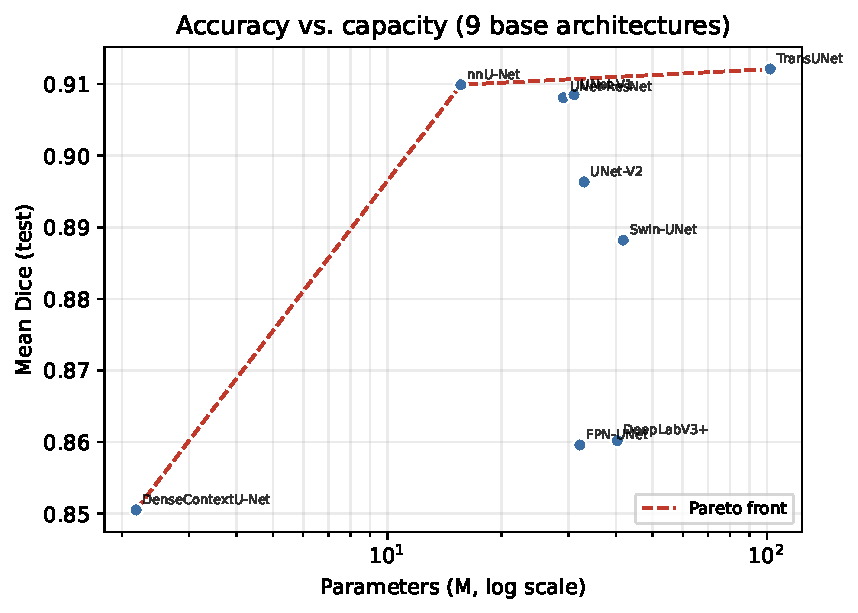
\includegraphics[width=0.92\linewidth]{figures/fig_pareto}
\caption{Accuracy--cost Pareto frontier. Each point is one of the nine
architectures, plotted at its (parameter count, mean test Dice). The
Pareto front is highlighted.}
\label{fig:pareto}
\end{figure}

%------------------------------------------------------------------------------
\subsection{Statistical significance}
\label{sec:results-significance}

We test all $\binom{9}{2}=36$ pairwise model differences on mean Dice with the
Wilcoxon signed-rank test, Bonferroni-corrected. The test is computed over the
$50$ patients rather than the $200$ frames. The frames are two views and two
phases of each patient, so treating them as independent observations inflates
the sample fourfold and lowers the bar for significance; the patient is the unit
about which any clinical claim is made. For transparency: on this benchmark the
choice changes nothing --- $27$ of the $36$ pairs are significant under either
unit --- because the differences that survive correction are far larger than the
extra power the wrong unit would buy. We report the patient-level test because
it is the correct estimand, not because it alters the outcome.

%==============================================================================
% Paper 1 / T7 — Wilcoxon (auto-generated)
%==============================================================================
\begin{table*}[t]
\centering
\caption{Pairwise Wilcoxon signed-rank test on mean Dice,
Bonferroni-corrected over $\binom{9}{2} = 36$ pairs. ``NS'' marks
pairs not significantly different at $p < 0.05$ after correction.
Tests are computed over the $50$ \emph{patients}, not the $200$ frames:
the frames are two views and two phases of each patient and are not
independent, so testing over them would inflate the sample fourfold.
On this table the correction changes no conclusion --- 27 of
36 pairs reach significance at frame level and 27 at
patient level, with 0 pairs differing --- because the surviving
differences are far larger than the extra power the wrong unit would buy.
We report the patient-level test because it is the correct estimand, not
because it alters the outcome.}
\label{tab:wilcoxon}
\small
\setlength{\tabcolsep}{3pt}
\resizebox{\textwidth}{!}{%
\begin{tabular}{l c c c c c c c c c }
\toprule
 & UNet-V1 & UNet-V2 & UNet-ResNet & DeepLabV3+ & nnU-Net & DenseContextU-Net & FPN-UNet & Swin-UNet & TransUNet \\
\midrule
UNet-V1 & --- & 7e-07 & NS & 3e-13 & NS & 6e-14 & 4e-13 & 2e-10 & NS \\
UNet-V2 &  & --- & 1e-05 & 1e-07 & 3e-07 & 7e-12 & 2e-09 & 4e-02 & 2e-07 \\
UNet-ResNet &  &  & --- & 2e-12 & NS & 6e-10 & 2e-13 & 4e-08 & NS \\
DeepLabV3+ &  &  &  & --- & 6e-13 & NS & NS & 2e-05 & 9e-13 \\
nnU-Net &  &  &  &  & --- & 1e-13 & 1e-13 & 1e-11 & NS \\
DenseContextU-Net &  &  &  &  &  & --- & NS & 6e-10 & 2e-13 \\
FPN-UNet &  &  &  &  &  &  & --- & 7e-08 & 6e-13 \\
Swin-UNet &  &  &  &  &  &  &  & --- & 7e-12 \\
TransUNet &  &  &  &  &  &  &  &  & --- \\
\bottomrule
\end{tabular}}
\end{table*}


\paragraph{Top-tier band.}
The nine non-significant pairs form exactly two cliques and nothing else. All
six pairs among the four highest-Dice architectures (TransUNet, nnU-Net,
UNet-ResNet, UNet-V1) are indistinguishable, as are all three among the lowest
(DeepLabV3+, FPN-UNet, Dense\-Context\-U-Net); every one of the remaining $27$ pairs
separates. The leaderboard is therefore better read as three tiers than as a
ranking of nine. Two of the three architectures in the lower clique are among
those whose training stopped early, so that grouping may reflect a shared
training artefact rather than a shared architectural limit. Full pairwise
$p$-values are released as supplementary data.

\paragraph{Small Dice gaps are within training variance.}
The differences separating the top-tier architectures are of order
$0.002$--$0.005$ Dice. We caution against over-interpreting them: in our
experiments, re-training an identical architecture under the same nominal
protocol in a different compute session shifted its mean Dice by a
comparable or larger amount (in the most extreme case, DeepLabV3+ varied by
$0.057$ between two runs). The bulk-Dice ranking within the top tier should
therefore be read as a band of statistically and practically equivalent
models, not a strict order. The architecturally meaningful differences in
this benchmark are the larger-magnitude ones: the boundary accuracy
(HD95), the clinical EF agreement, and the efficiency trade-off,
discussed in Section~\ref{sec:discussion}.

The critical-difference diagram of Figure~\ref{fig:cd} renders the
banding visually: architectures joined by a horizontal bar are not
significantly different in average per-sample rank. Here average rank
tracks mean Dice closely --- the two orderings agree for all nine
architectures --- and TransUNet leads on both, with an average rank of
$2.96$ across the $200$ test frames against nnU-Net's $3.10$.

Aggregating to the $50$ patients before ranking, which is the correct
inferential unit given that the $200$ frames are four views and phases of
each patient, leaves TransUNet first ($2.68$) but exchanges second and
third between nnU-Net ($2.92$) and UNet-V1 ($2.82$). The four leading
architectures span only $0.37$ of a rank at the frame level and fall
inside a single clique, and their order is not stable to the choice of
aggregation unit. Both observations point the same way: the top tier is a
statistically equivalent band, not a ranking.

\begin{figure}[t]
\centering
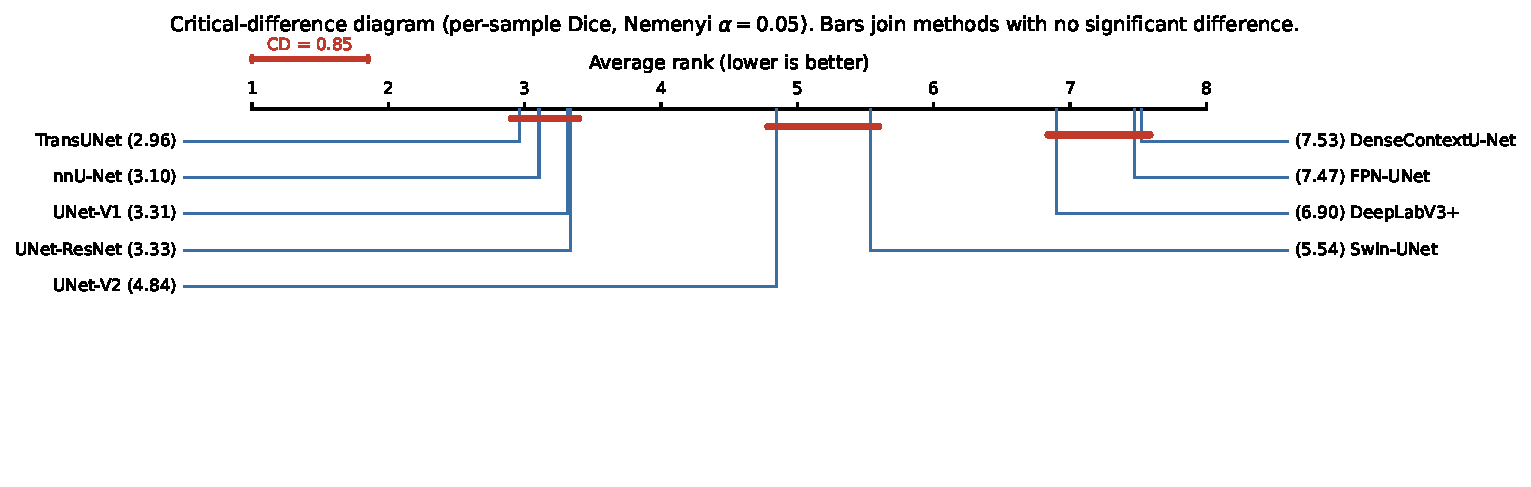
\includegraphics[width=0.95\linewidth]{figures/fig_cd_diagram}
\caption{Critical-difference diagram (average ranks on per-sample Dice,
Nemenyi test, $\alpha = 0.05$). Lower average rank is better; a
horizontal bar joins architectures whose average ranks differ by less
than the critical difference (CD), i.e.\ that are not significantly
different.}
\label{fig:cd}
\end{figure}

%------------------------------------------------------------------------------
\subsection{Qualitative results}
\label{sec:results-qualitative}

Figure~\ref{fig:qualitative} shows sample predictions from the top four
architectures plus a bottom-tier representative on three patients spanning
the Good / Medium / Poor image-quality grades.

\begin{figure}[p]
\centering
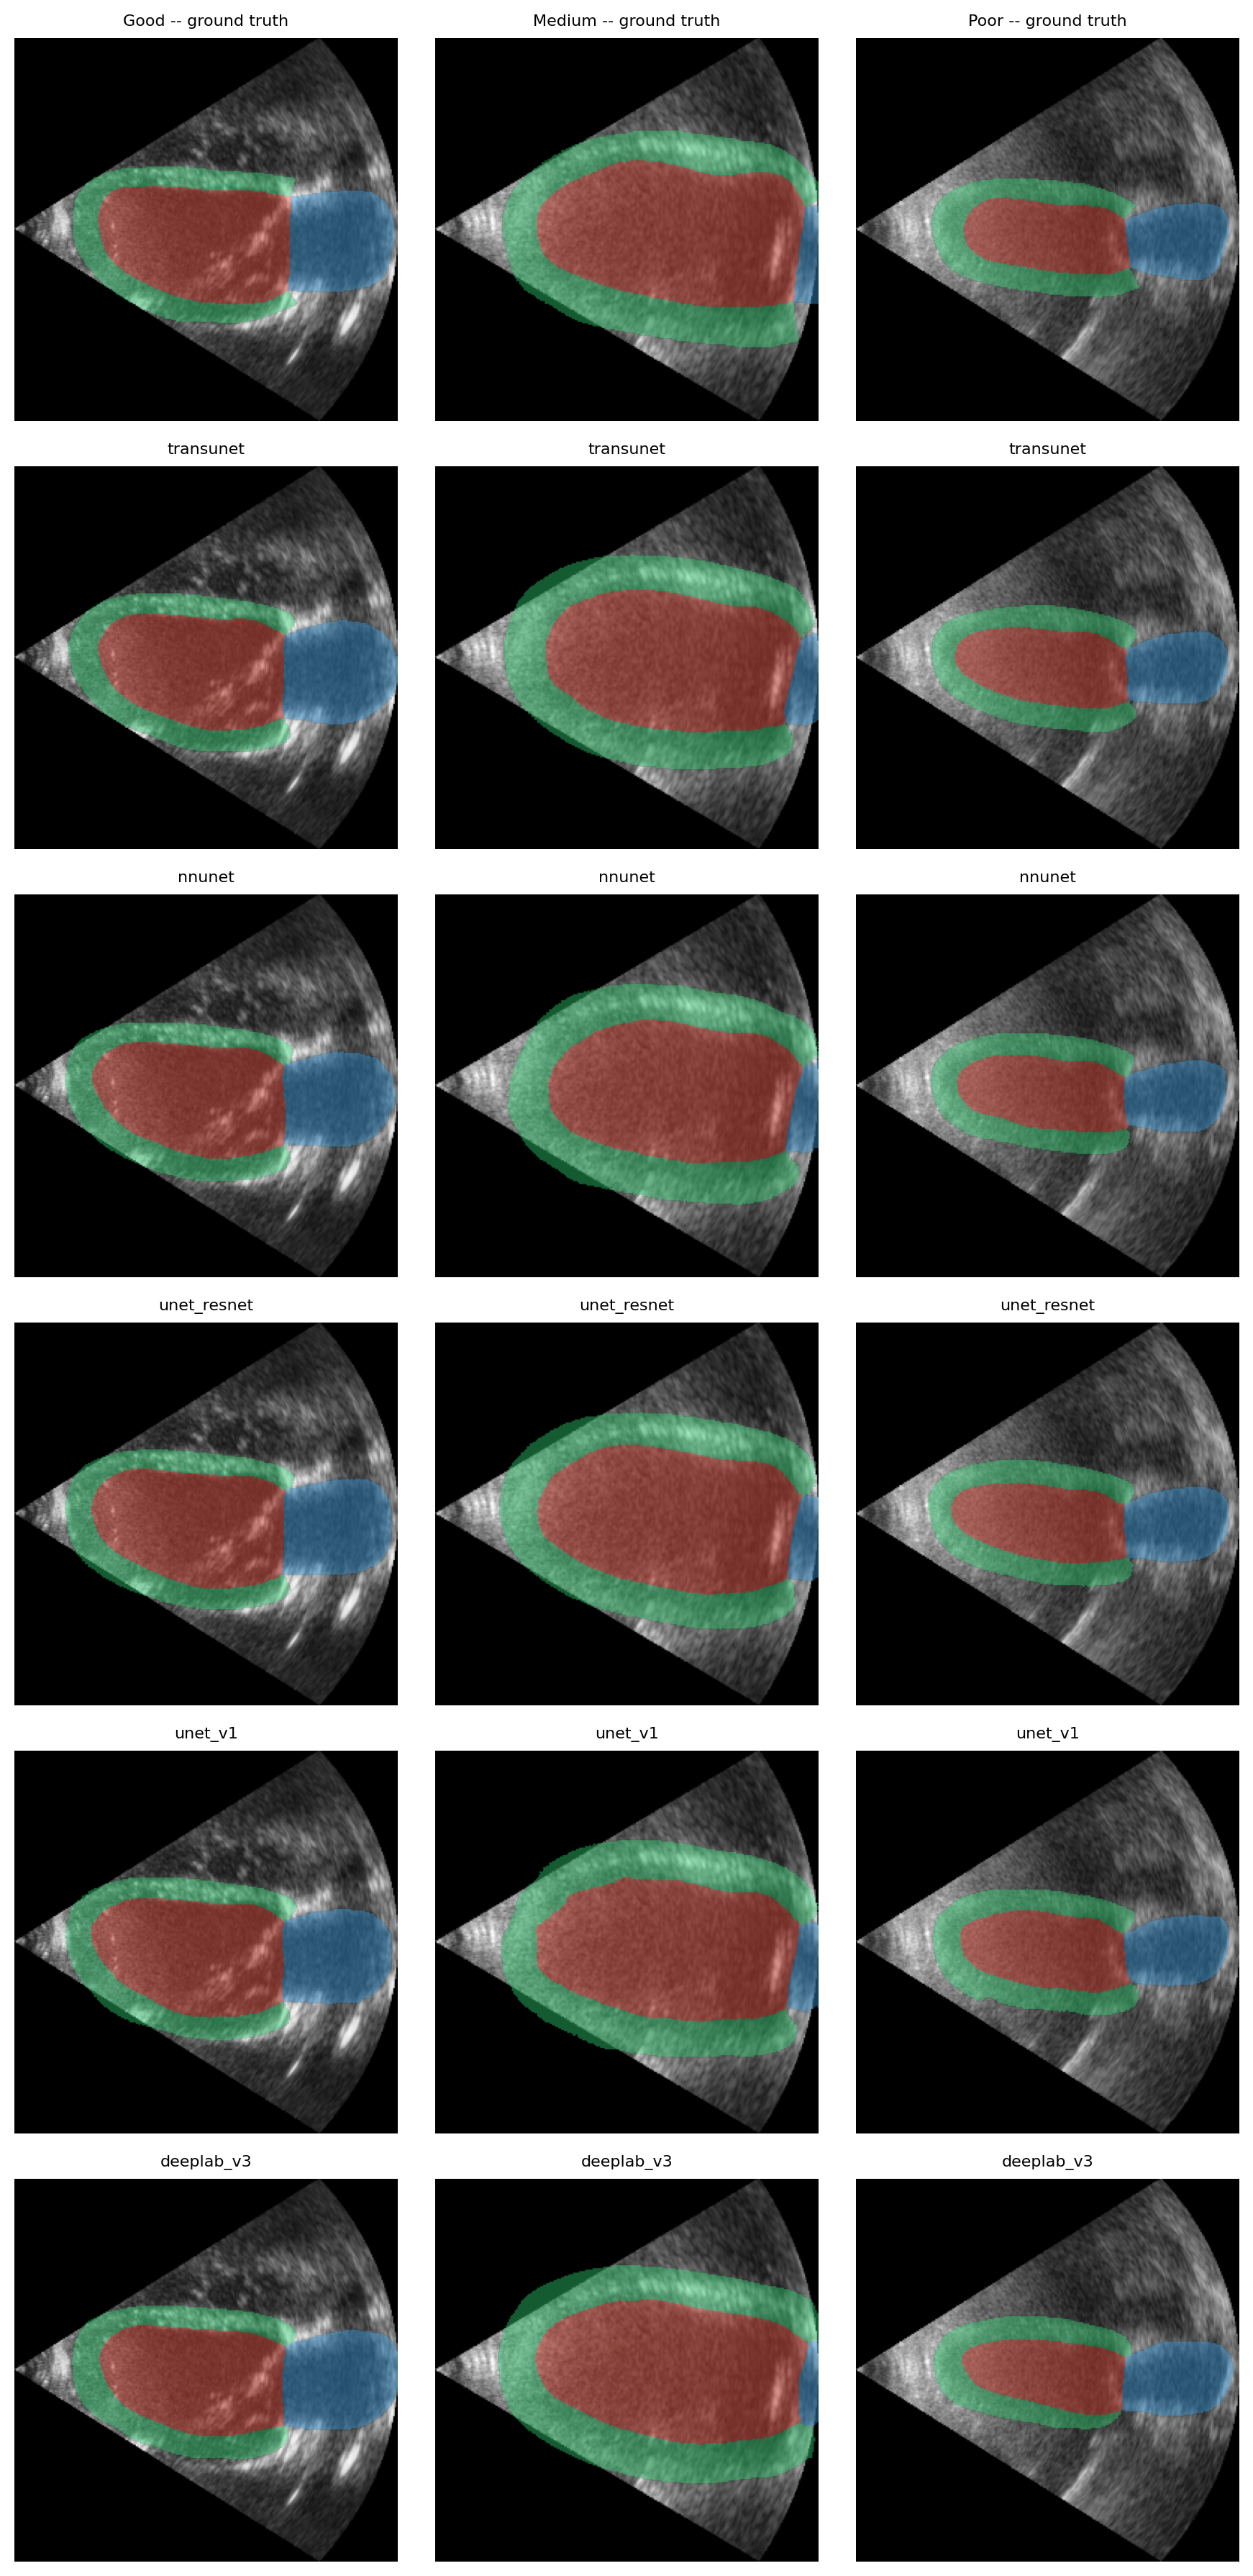
\includegraphics[height=0.9\textheight]{figures/fig_qualitative}
\caption{Qualitative predictions on three test patients spanning the Good,
Medium, and Poor image-quality grades (columns). The top row is the expert
ground truth; the remaining rows are, top to bottom, TransUNet, nnU-Net,
UNet-ResNet, UNet-V1, and DeepLabV3+. Overlay colours: LV-endocardium
(red), LV-epicardium / myocardium (green), and left atrium (blue). Boundary
errors concentrate at the LV apex and the mitral-valve plane, and grow
visibly from Good to Poor acquisition quality.}
\label{fig:qualitative}
\end{figure}
